% !TeX root = ../../../../../thesis.tex


\subsubsection{SMPS and LED}

In \autoref{fig:ac-smps-led-and-smps-picture} a commercial LED lighting fixture can be seen with a switching mode power supply (SMPS).
The power supply transforms the AC to a DC signal which is used to power the LED.




For this setup we investigate what the current signature looks like when the LED is on, representing a `1', and when the LED is off,  representing a `0'.
A 10 ohm resistor is placed in series with the SMPS on the AC side and the voltage drop over this resistor is measured.
So a voltage is measured, but the current that flows can be calculated using Ohm's law: $I = \frac{U}{R}$.
Since we are investigating how the current signature behaves, it is not needed to have exact numbers on the current draw.








\begin{figure}[b]
	\centering     %%% not \center
	\subfigure[Encoding a `0', LED off.]{
		\label{fig:smps-current-primary-no-load}
		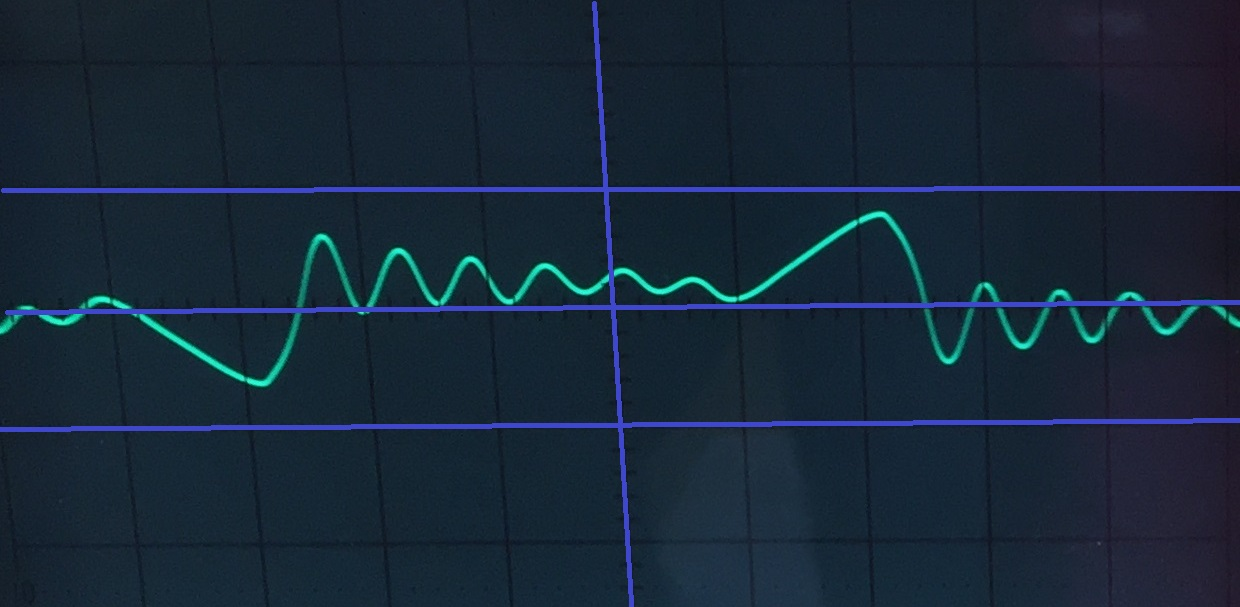
\includegraphics[width=60mm]
		{chapters/hardware-chapters/AC/ac-modulator/smps-led/smps-current-primary-no-load-cropped-edit.jpg}
	}
	\subfigure[Encoding a `1', LED on.]{ 
		% 33 ohm...
		\label{fig:smps-current-primary-with-load}
		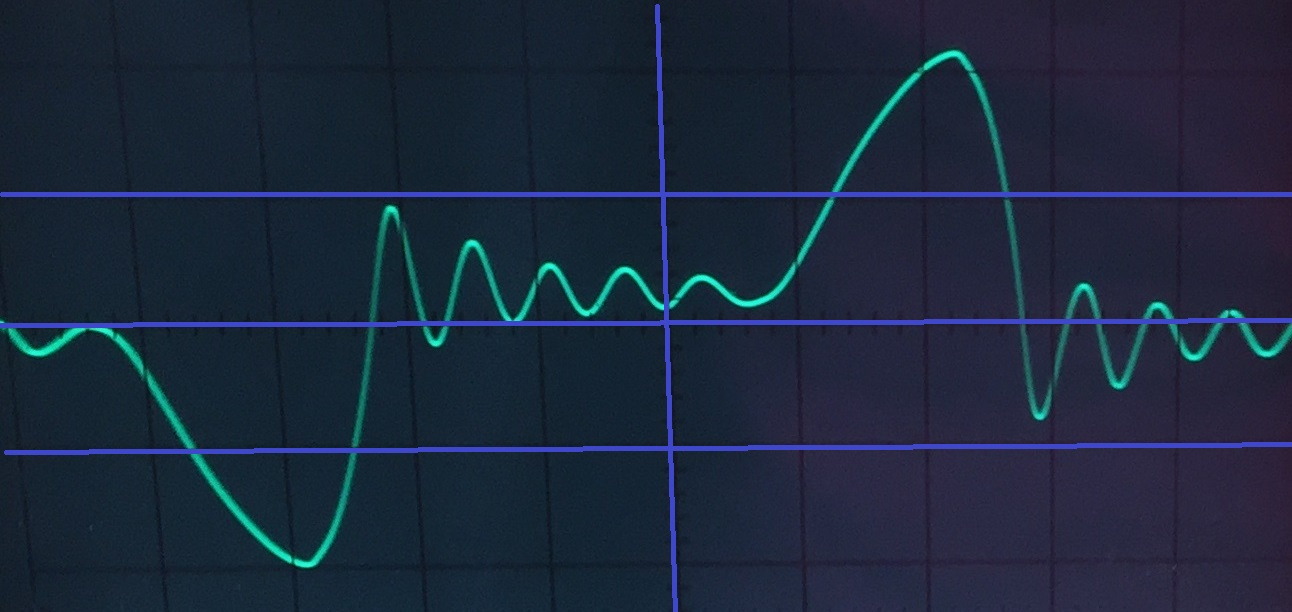
\includegraphics[width=60mm]
		{chapters/hardware-chapters/AC/ac-modulator/smps-led/smps-current-primary-with-load-cropped-edit.jpg}
	}

	\caption{Voltage measured over a 10 ohm series resistor at the primary side, to determine the current flow in two situations of a SMPS, when encoding a `0' and a `1'. X-axis: 2 ms/div, Y-axis: 500 mV/div.}
\end{figure}






In Figures \ref{fig:smps-current-primary-no-load} and \ref{fig:smps-current-primary-with-load} the current signature of the SMPS can be seen, when encoding a `0' (LED off) and when encoding a `1' (LED on), respectively.
From these figures, it is clear to see that when encoding a zero, the current is not zero and when encoding a `1', the current is not a constant value.
This makes it difficult to determine what the ID of the transmitting LED is.
This becomes even more difficult when multiple of these current signatures get superimposed.



